\documentclass[letterpaper,12pt]{article}

\usepackage{fontspec}
\usepackage{microtype} % Better typography
\usepackage{mathpazo} % for palatino math

\setmainfont{Lyon Text}\linespread{1.15}
%\setmainfont{Guardian TextEgyp}\linespread{1.15}
%\setmainfont{Goudy Oldstyle Std}\linespread{1.15}
%\setmainfont{Minion Pro}\linespread{1.15}

\setsansfont[BoldFont={Helvetica Neue Medium}]{Helvetica Neue}
%\setsansfont[BoldFont={Guardian TextEgyp Medium}]{Guardian TextEgyp}
%\setsansfont[BoldFont={Myriad Pro}]{Myriad Pro Light}

%\setmonofont{Menlo}


% PAGE MARGINS
\usepackage[margin=1.33in]{geometry}

\tolerance=5000

% PARAGRAPH SPACING
\setlength{\parskip}{2.0ex}
\setlength{\parindent}{0ex}

% LISTS
\usepackage{enumitem}
\setenumerate{noitemsep,nolistsep}
\setitemize{noitemsep,nolistsep}

% SECTIONS AND CHAPTER HEADINGS FORMATTING
\usepackage[compact,noindentafter]{titlesec}
\titleformat*{\section}{\sffamily\large\bfseries}
\titlespacing{\section}{0pt}{1.5ex}{0ex}
\titleformat*{\subsection}{\sffamily\normalsize\bfseries}
\titlespacing{\subsection}{0pt}{1ex}{0ex}

\setlength{\headheight}{14.49998pt}

% ------- CUSTOM TITLE FORMAT -------
%
\makeatletter
\renewcommand{\maketitle}{
\begin{flushleft}          % right align
{\Large\sffamily\bfseries\@title}   % increase the font size of the title
\vspace{2ex}\\            % vertical space between the title and author name
{\normalsize\sffamily\@author}           % author name
\vspace{0ex}\\             % vertical space between author name and date
\small\sffamily\@date                     % date
\vspace{5ex}              % vertical space between the author block and abstract
\end{flushleft}
}
% -----------------------------------

% BIBLIOGRAPHY
\usepackage{natbib}                  % for our chosen bibliography style




%------------------------------------------------------------------------------
%	TITLE & AUTHORS & AFFILIATIONS
%------------------------------------------------------------------------------

\title{This is the title of the manuscript}

\author[1,2,3,*]{Paul L. Gribble}
\author[1,2,4]{Ford Prefect}

\affil[1]{The Brain and Mind Institute, The University of Western Ontario}
\affil[2]{Department of Psychology, The University of Western Ontario}
\affil[3]{Department of Physiology \& Pharmacology, Schulich School of Medicine \& Dentistry}
\affil[4]{Graduate Program in Neuroscience, The University of Western Ontario}

\begin{document}

\begin{singlespace}
\nolinenumbers

\maketitle
\thispagestyle{empty}

\hfill

\begin{flushleft}

%------------------------------------------------------------------------------
%	MAILING ADDRESS & CORRESPONDING AUTHOR INFO
%------------------------------------------------------------------------------

\vspace{35mm}
$^{*}$\textbf{Corresponding Author}\\
\vspace{2ex}
Professor Paul Gribble\\
The Brain and Mind Institute, Dept. Psychology\\
1151 Richmond St, NSC Bldg Room 120\\
London, Ontario, Canada N6A 5B7\\
Phone: +1 519.661.2111 ext. 82237\\
Fax: +1 519.661.3613\\
email: \url{paul@gribblelab.org}

%------------------------------------------------------------------------------
%	KEYWORDS
%------------------------------------------------------------------------------

\vfill
\textbf{Keywords}: blah; blah blah; blah blah blah\\

\vspace{3ex}
{\emph{\today, \currenttime}}

\end{flushleft}

\end{singlespace}

%------------------------------------------------------------------------------
%	ABSTRACT
%------------------------------------------------------------------------------

\newpage
\linenumbers

\section*{Abstract}

\lipsum[1]

%------------------------------------------------------------------------------
%	INTRODUCTION
%------------------------------------------------------------------------------

\newpage
\section*{Introduction}

Blah blah blah lots of crazy research has been done on this topic \citep{Mattar:2005}. Blah blah blah lots of crazy research has been done\footnote{ya ya w8ever} on this topic \citep{Mattar:2005}. Blah blah blah lots of crazy research has been done on this topic \citep{Mattar:2005}. \lipsum[1]

\lipsum[1-3]

%------------------------------------------------------------------------------
%	METHODS
%------------------------------------------------------------------------------

\section*{Methods}

\lipsum[1-2] See equation~\ref{eq:line} for some junk.

\begin{equation}
\hat{Y_{i}} = \beta_{0} + \beta_{1} X_{i} + \epsilon_{i}
\label{eq:line}
\end{equation}

Also see Figure~\ref{fig:setupfig} for some other junk.

\lipsum[1-3]

%------------------------------------------------------------------------------
%	RESULTS
%------------------------------------------------------------------------------

\section*{Results}

Table~\ref{tbl:somedata} is totally meaningless.
\lipsum[1-5]

%------------------------------------------------------------------------------
%	DISCUSSION
%------------------------------------------------------------------------------

\section*{Discussion}

\lipsum[1-8]

%------------------------------------------------------------------------------
%	ACKNOWLEDGEMENTS
%------------------------------------------------------------------------------

\newpage
\section*{Acknowledgements}
This research was supported by grants to PLG by the Canadian Institutes of Health Research and the Natural Sciences and Engineering Council of Canada.

%------------------------------------------------------------------------------
%	REFERENCES
%------------------------------------------------------------------------------

\newpage
\nolinenumbers

\bibliographystyle{jneurosci} 
%\bibliographystyle{jneurophysiol}
\bibliography{refs}

%------------------------------------------------------------------------------
%	TABLES
%------------------------------------------------------------------------------

\newpage
\clearpage
\parbox[c][\textheight][s]{\linewidth}{%
\begin{table}[H]
	\centering
	\begin{tabular}{c|c}
		condition &mean\\
		\hline\hline
		A         &10.1\\
		B         &11.0\\
	\end{tabular}
 \caption{Blah blah some data.}
 \label{tbl:somedata}
\end{table}
}

%------------------------------------------------------------------------------
%	FIGURES
%------------------------------------------------------------------------------

\newpage
\clearpage
\parbox[c][\textheight][s]{\linewidth}{%
\begin{figure}[H]
	\centering
    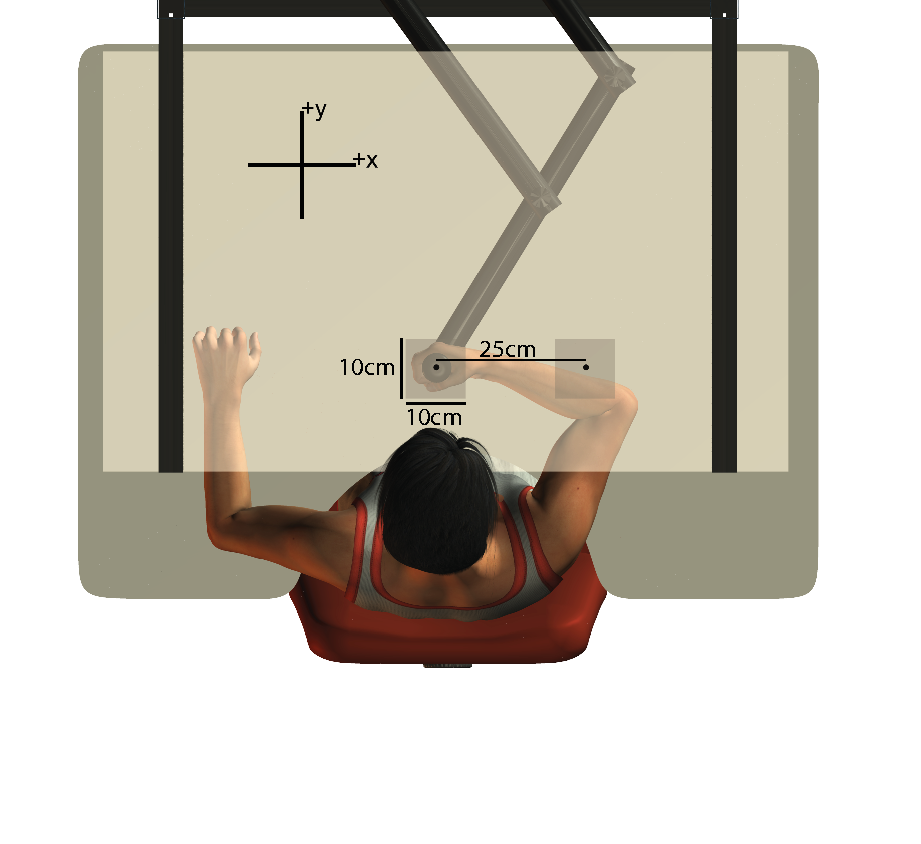
\includegraphics[height=3in]{figure1.pdf}
 \caption{Blah blah blah the robot setup blah.}
 \label{fig:setupfig}
\end{figure}
}

\end{document}

